\documentclass[a4paper,14pt]{extarticle}

% Путь до папки с общими шаблонами
\newcommand{\pathToCommonFolder}{/home/denilai/Documents/repos/latex/Common}
% Название работы в титуле
\newcommand{\workname}{Практическая работа №2}
% Название дисциплины в титуле
\newcommand{\discipline}{Техническое обслуживание\\программно--аппаратных комплексов}
% Название кафедры в титуле
\newcommand{\kafedra}{Кафедры Вычислительной техники}
% Тема работы в титуле
\newcommand{\theme}{}
\newcommand{\dontneedtheme}{1}
% Должность преподавателя в титуле
\newcommand{\rang}{ассистент }
% ФИО студента в титуле
\newcommand{\studentfio}{К.~Ю.~Денисов}
% ФИО преподавателя в титуле
\newcommand{\teacherfio}{Л.~В.~Скоропупов}
\newcommand{\signature}{\pathToCommonFolder/empty}


Мои курсы
_51
\usepackage{tabularx}


\usepackage{booktabs}
%\newcolumntype{b}{X}
%\newcolumntype{s}{>{\hsize=.5\hsize}X}
\newcommand{\heading}[1]{\multicolumn{1}{c}{#1}}

% установка размера шрифта для всего документа
%\fontsize{20pt}{18pt}\selectfont
\usepackage{extsizes} % Возможность сделать 14-й шрифт

% Вставка заготовки преамбулы
% Этот шаблон документа разработан в 2014 году
% Данилом Фёдоровых (danil@fedorovykh.ru) 
% для использования в курсе 
% <<Документы и презентации в \LaTeX>>, записанном НИУ ВШЭ
% для Coursera.org: http://coursera.org/course/latex .
% Исходная версия шаблона --- 
% https://www.writelatex.com/coursera/latex/5.3

% В этом документе преамбула

% Для корректного использования русских символов в формулах
% пакеты hyperref и настройки, связанные с ним, стоит загуржать
% перед загрузкой пакета mathtext



% поддержка русских букв
% кодировка шрифта
%\usepackage[T2A]{fontenc} 
\usepackage{pscyr}

% использование ненумеровонного абзаца с добавлением его в содержаниеl

\newcommand{\anonsection}[1]{\section*{#1}\addcontentsline{toc}{section}{#1}}
\newcommand{\sectionunderl}[1]{\section*{\underline{#1}}}


% настройка окружения enumerate
\usepackage{enumitem}
\setlist{noitemsep}
\setlist[enumerate]{labelsep=*, leftmargin=1.5pc}

\usepackage{hyperref}

% сначала ставить \usepackage{extsizes} % Возможность сделать 14-й шрифт
% для корректной установки полей вставлять преамбулу следует в последнюю очередь (но перед дерективой замены \rmdefault)
\usepackage[top=20mm,bottom=25mm,left=35mm,right=20mm]{geometry} % Простой способ задавать поля

\hypersetup{				% Гиперссылки
	unicode=true,           % русские буквы в раздела PDF
	pdftitle={Заголовок},   % Заголовок
	pdfauthor={Автор},      % Автор
	pdfsubject={Тема},      % Тема
	pdfcreator={Создатель}, % Создатель
	pdfproducer={Производитель}, % Производитель
	pdfkeywords={keyword1} {key2} {key3}, % Ключевые слова
	colorlinks=true,       	% false: ссылки в рамках; true: цветные ссылки
	linkcolor=red,          % внутренние ссылки
	citecolor=black,        % на библиографию
	filecolor=magenta,      % на файлы
	urlcolor=blue           % на URL
}

%%% Работа с русским языком
\usepackage{cmap}					% поиск в PDF
\usepackage{mathtext} 				% русские буквы в формулах
\usepackage[T2A]{fontenc}			% кодировка
\usepackage[utf8]{inputenc}			% кодировка исходного текста
\usepackage[english,russian]{babel}	% локализация и переносы
\usepackage{indentfirst}
\frenchspacing

%для изменения названия списка иллюстраций
\usepackage{tocloft}


\renewcommand{\epsilon}{\ensuremath{\varepsilon}}
\renewcommand{\phi}{\ensuremath{\varphi}}
\renewcommand{\kappa}{\ensuremath{\varkappa}}
\renewcommand{\le}{\ensuremath{\leqslant}}
\renewcommand{\leq}{\ensuremath{\leqslant}}
\renewcommand{\ge}{\ensuremath{\geqslant}}
\renewcommand{\geq}{\ensuremath{\geqslant}}
\renewcommand{\emptyset}{\varnothing}

% Изменения параметров списка иллюстраций
\renewcommand{\cftfigfont}{Рисунок } % добавляем везде "Рисунок" перед номером
\addto\captionsrussian{\renewcommand\listfigurename{Список иллюстративного материала}}

\newcommand{\tm}{\texttrademark\ }
\newcommand{\reg}{\textregistered\ }


%%% Дополнительная работа с математикой
\usepackage{amsmath,amsfonts,amssymb,amsthm,mathtools} % AMS
\usepackage{icomma} % "Умная" запятая: $0,2$ --- число, $0, 2$ --- перечисление

%% Номера формул
%\mathtoolsset{showonlyrefs=true} % Показывать номера только у тех формул, на которые есть \eqref{} в тексте.
%\usepackage{leqno} % Нумереация формул слева

%% Свои команды
\DeclareMathOperator{\sgn}{\mathop{sgn}}

%% Перенос знаков в формулах (по Львовскому)
\newcommand*{\hm}[1]{#1\nobreak\discretionary{}
{\hbox{$\mathsurround=0pt #1$}}{}}


% отступ для первого абзаца главы или параграфа
%\usepackage{indentfirst}

%%% Работа с картинками
\usepackage{graphicx}  % Для вставки рисунков
\graphicspath{{images/}{screnshots/}}  % папки с картинками
\DeclareGraphicsExtensions{.pdf,.png,.jpg}
\setlength\fboxsep{3pt} % Отступ рамки \fbox{} от рисунка
\setlength\fboxrule{1pt} % Толщина линий рамки \fbox{}
\usepackage{wrapfig} % Обтекание рисунков текстом

%%% Работа с таблицами
\usepackage{array,tabularx,tabulary,booktabs} % Дополнительная работа с таблицами
\usepackage{longtable}  % Длинные таблицы
\usepackage{multirow} % Слияние строк в таблице

%%% Теоремы
\theoremstyle{plain} % Это стиль по умолчанию, его можно не переопределять.
\newtheorem{theorem}{Теорема}[section]
\newtheorem{proposition}[theorem]{Утверждение}

\theoremstyle{plain} % Это стиль по умолчанию, его можно не переопределять.
\newtheorem{work}{Практическая работа}[part]


 
 
\theoremstyle{definition} % "Определение"
\newtheorem{corollary}{Следствие}[theorem]
\newtheorem{problem}{Задача}[section]
 
\theoremstyle{remark} % "Примечание"
\newtheorem*{nonum}{Решение}



%%% Программирование
\usepackage{etoolbox} % логические операторы

%%% Страница

%	\usepackage{fancyhdr} % Колонтитулы
% 	\pagestyle{fancy}
%   \renewcommand{\headrulewidth}{0pt}  % Толщина линейки, отчеркивающей верхний колонтитул
% 	\lfoot{Нижний левый}
% 	\rfoot{Нижний правый}
% 	\rhead{Верхний правый}
% 	\chead{Верхний в центре}
% 	\lhead{Верхний левый}
%	\cfoot{Нижний в центре} % По умолчанию здесь номер страницы

\usepackage{setspace} % Интерлиньяж
\onehalfspacing % Интерлиньяж 1.5
%\doublespacing % Интерлиньяж 2
%\singlespacing % Интерлиньяж 1

\usepackage{lastpage} % Узнать, сколько всего страниц в документе.

\usepackage{soul} % Модификаторы начертания


\usepackage[usenames,dvipsnames,svgnames,table,rgb]{xcolor}


\usepackage{csquotes} % Еще инструменты для ссылок

%\usepackage[style=authoryear,maxcitenames=2,backend=biber,sorting=nty]{biblatex}

\usepackage{multicol} % Несколько колонок

\usepackage{tikz} % Работа с графикой
\usepackage{pgfplots}
\usepackage{pgfplotstable}

% модуль для вставки рыбы
\usepackage{blindtext}

\usepackage{listings}
\usepackage{color}


% для поворота отдельной страницы. Использовать окружение \landscape
\usepackage{pdflscape} 
\usepackage{rotating} 


\definecolor{mygreen}{rgb}{0,0.6,0}
\definecolor{mygray}{rgb}{0.5,0.5,0.5}
\definecolor{mymauve}{rgb}{0.58,0,0.82}


% пример импорта файла
%\lstinputlisting{/home/denilai/repomy/conf/distributions}

\lstset{
	language=Python,
	basicstyle=\footnotesize,        % the size of the fonts that are used for the code
	numbers=left,                    % where to put the line-numbers; possible values are (none, left, right)
	numbersep=5pt,                   % how far the line-numbers are from the code
	numberstyle=\tiny\color{mygray}, % the style that is used for the line-numbers
	stepnumber=2,                    % the step between two line-numbers. If it's 1, each line will be numbered
	% Tab - 2 пробела
	tabsize=2,    
	% Автоматический перенос строк
	breaklines=true,
	frame=single,
	breakatwhitespace=true,
	title=\lstname 
}


%\usepackage[top=20mm,bottom=20mm,left=20mm,right=15mm]{geometry} % Простой способ задавать поля

\author{Кирилл Денисов}
\title{Практическая работа №4}
\date{\today}

\renewcommand{\withouttheme}{1}

% установка полуторного интервала
% \usepackage{setspace}  
% \onehalfspacing

% использовать Times New Roman
\renewcommand{\rmdefault}{ftm}


\begin{document}
	\thispagestyle{empty}
	% Вставка первого титульного листа
	%\newcommand{\withouttheme}{} добавить эту переменную для определения, нужна ли тема
%     {} - нужна
%    {1} - не нужна

%\newcommand{\withoutsubmissiondate}{} добавить эту переменную для определения, нужен ли срок предоставления отчета
%     {} - нужен
%    {1} - не нужен
\begin{center}
	\begin{figure}[h!]
		\begin{center}
		
\includegraphics[width=0.17\linewidth]{\pathToCommonFolder/gerb}
		%\caption{}\label{pic:first}
		%	\vspace{5ex}
		\end{center}	
	\end{figure}
 	\small	МИНОБРНАУКИ РОССИИ \\
	Федеральное государственное бюджетное образовательное учреждение\\
						высшего профессионального образования\\
\normalsize					
\textbf{«МИРЭА – Российский технологический университет»\\
						РТУ МИРЭА}\\
						\noindent\rule{1\linewidth}{1pt}\\
       Институт информационных технологий\\ %\vspace{2ex}
					\kafedra\\
		\vspace{3ex}
			\large \textbf{\workname}  \\
		%\vspace{1ex}
						по дисциплине\\ «\discipline» \\
		\vspace{3ex}
		\if \withouttheme
			\textbf{Тема работы:}\\ <<\theme>>
		\fi
\vspace{3ex}
\small
\begin{table}[h!]
\begin{tabular}{p{0.14\linewidth}p{0.38\linewidth}p{0.25\linewidth}p{0.2\linewidth}}
	\textbf{Выполнил:} & студент группы ИВБО-02-19 & \studentfio &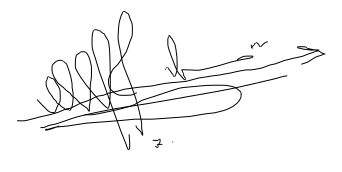
\includegraphics[width=0.8\linewidth]{\signature}\\ \\
	\textbf{Принял:} & \rang & \teacherfio 
\end{tabular}
\end{table}
\end{center}

\begin{flushleft}
	\begin{tabular}{p{0.25\linewidth}l}

		Работа выполена & <<\noindent\rule{2em}{1pt}>>
		                    \noindent\rule{5em}{1pt} 202\noindent\rule{1em}{1pt} \\

		<<Зачтено>> & <<\noindent\rule{2em}{1pt}>>
		\noindent\rule{5em}{1pt} 202\noindent\rule{1em}{1pt} \\

	\end{tabular}
\end{flushleft}

\normalsize
\begin{center}	
\vfill 
Москва 2021
\end{center}

	\newpage
%	\tableofcontents
	\newpage
%	\listoftables
	
	
	
	
\section*{Постановка задачи}

Произвести расчет численности работников, занятых
сервисным обслуживанием и текущим
ремонтом СВТ (средств вычислительной
техники) согласно варианту.




\section*{Индивидуальный вариант №6}

\begin{table}[htbp]
	
	\small
	\begin{tabular}{|p{0.1\linewidth}|p{0.12\linewidth}|p{0.12\linewidth}|p{0.12\linewidth}|p{0.12\linewidth}|p{0.12\linewidth}|p{0.12\linewidth}|}
		\hline
		№
		Варианта & Кол-во
		ПК & Кол-во
		лазерных
		принтеров & Кол-во
		струйных
		принтеров & Текущий ремонт & Научно-технические услуги & Заказ и получение оборудования \\ \hline
		\multicolumn{1}{|r|}{6} & \multicolumn{1}{r|}{4} & \multicolumn{1}{r|}{1} & \multicolumn{1}{r|}{1} & \multicolumn{1}{r|}{0} & \multicolumn{1}{r|}{2} & \multicolumn{1}{r|}{1} \\ \hline
	\end{tabular}
    \caption{Индивидуальный вариант №6}
	\label{}
\end{table}


\section*{Ход работы}

Приведем объем ремонтно-профилактических работ по ежедневному, ежемесячному и полугодовому обслуживанию ПК (см. таблицу \ref{tab:pc})

\begin{table}[htbp]
	\scriptsize
	\caption{Ремонтно-профилактические работы с ПК}
	\begin{tabular}{|m{0.02\linewidth}|m{0.4\linewidth}|m{0.14\linewidth}|m{0.1\linewidth}|m{0.1\linewidth}|m{0.1\linewidth}|}
		\hline
		№ & Вид выполняемой работы & Единица измерения & Объем работы за год в единицах измерения & Норма времени на единицу измерения. ч.& Нормативные затраты времени на объем работ. ч. \\\hline
		\multicolumn{ 6}{|c|}{Еженедельное обслуживание} \\ \hline
		1 & Проверка работоспособности устройств на тестах в ускоренном режиме&одно устройство
		&208&	0.13&	27.04
			\\ \hline
		2 & Очистка магнитных головок устройств внешней памяти (накопители на гибких магнитных дисках) & одна головка & 208	&0.09&	18.72
		 \\  \hline
		3 & Проверка и удаление компьютерных вирусов на устройствах внешней памяти ПК & Один ПК & 208&	0.2	&41.6
		 \\ \hline
		4 & Проведение дефрагментации накопителей на жестких магнитных дисках & один накопитель & 208&	0.27&	56.16
		 \\ \hline
		\multicolumn{6}{|c|}{Ежемесячное обслуживание} \\ \hline
		5 & Полное тестирование всех устройств ПК с выдачей протокола. в том числе и ЛВС. выявление и исправление ошибок в распределении дискового пространства &	Один ПК	&48	&1.7&	81.6
		 \\ \hline
		6 & Поставка обновленных антивирусных программ и полная проверка дисковой памяти на наличие вирусов & Один ПК & 48&	0.48&	23.04
		 \\ \hline
		7 & Очистка от пыли внутренних объемов ПК с разборкой & Один ПК &48&	0.37&	17.76
		 \\ \hline
		\multicolumn{ 6}{|c|}{Полугодовое обслуживание для персональных компьютеров (ПК) и периферийного оборудования} \\ \hline
		8	&Очистка от пыли внутренних объемов блоков питания ПК. очистка и смазка вентиляторов&	Один ПК&	8&	0.8&	6.4
		\\\hline
	\end{tabular}
	\label{tab:pc}
\end{table}

\newpage
\textbf{Струйный принтер}

Приведем объем ремонтно-профилактических работ по ежедневному, ежемесячному и полугодовому обслуживанию струйного принтера (см. таблицу \ref{tab:ink})
\begin{table}[h!]
	\scriptsize
	\caption{Ремонтно-профилактические работы с струйными принтерами}
	\begin{tabular}{|m{0.02\linewidth}|m{0.4\linewidth}|m{0.14\linewidth}|m{0.1\linewidth}|m{0.1\linewidth}|m{0.1\linewidth}|}
		\hline
		№ & Вид выполняемой работы & Единица измерения & Объем работы за год в единицах измерения & Норма времени на единицу измерения. ч.& Нормативные затраты времени на объем работ. ч. \\\hline
		
		\multicolumn{6}{|c|}{Ежемесячное обслуживание} \\ \hline
		
		1	&Очистка и промывка печатающих головок матричных и струйных принтеров&	один принтер&	52&	0.17&	8.84
		\\ \hline
		2&	Смазка механических устройств ТС (НГМД. стримеры. принтеры)	&одно устройство&	52	&0.34&	17.68
	\\ \hline
	\end{tabular}
	\label{tab:ink}
\end{table}


\textbf{Лазерный принтер}

Приведем объем ремонтно-профилактических работ по ежедневному, ежемесячному и полугодовому обслуживанию лазерного принтера (см. таблицу \ref{tab:jet})
\begin{table}[h!]
	\scriptsize
	\caption{Ремонтно-профилактические работы с лазерными принтерами}
	\begin{tabular}{|m{0.02\linewidth}|m{0.4\linewidth}|m{0.14\linewidth}|m{0.1\linewidth}|m{0.1\linewidth}|m{0.1\linewidth}|}
		\hline
		№ & Вид выполняемой работы & Единица измерения & Объем работы за год в единицах измерения & Норма времени на единицу измерения. ч.& Нормативные затраты времени на объем работ. ч. \\\hline
		
		\multicolumn{6}{|c|}{Ежемесячное обслуживание} \\ \hline
		
		1	&Смазка механических устройств ТС (НГМД. стримеры. принтеры)&	одно устройство	&52	&0.34&	17.68
		\\ \hline
		2	&	Очистка от неиспользованного тонера элементов печати лазерных принтеров. очистка и промывка оптики и своевременная заправка тонера&	один принтер&52	&0.34&	17.68\\ \hline
		
	\end{tabular}
	\label{tab:jet}
\end{table}

\textbf{Проведем расчет численности работников, занятых сервисным обслуживанием СВТ}

Нормативные затраты времени на объем работ за год составляют: 
\begin{align*}
	Т_р=Т_{рн}+Т_{рм}+Т_{рп} = 143.52 ч+	184.28 ч+	6.4 ч = 334.2 ч, \text{, где}
\end{align*} 
$Т_{рн}$ – нормативы времени на еженедельный вид работ,\\ $Т_{рм}$ – нормативы времени на ежемесячный вид работ,\\ $Т_{рп} $– нормативы времени на полугодовой вид работ.
Расчетная численность работников, занятых обслуживанием ПК, равна: 
\begin{align*}
		Т_р * k = 334.2ч* 1.08 = 360.94 ч
\end{align*}

Требуемая среднесписочная численность работников, занятых обслуживанием ПК, равна: 
\begin{align*}
	360.94 ч \div 2000  = 0.180468\approx 1 чел.
\end{align*}
Штатная численность составляет 1 сотрудник.


\paragraph*{Вывод}
Результатом практической работы является расчет численности работников, необходимой для выполнения всего объема работ.
\newpage
\anonsection{СПИСОК ИСПОЛЬЗУЕМЫХ ИСТОЧНИКОВ И ЛИТЕРАТУРЫ}
\begin{enumerate}
	\item Лекции по Техническому обслуживанию программно-аппаратных комплексов / Супруненко Д.В. --- МИРЭА, 2021.
	\item Методические указания по выполнению практических работ / МИРЭА --- Российский технологический университет.
	\item Постановление № 28 Об утверждении межотраслевых типовых норм времени на работы по сервисному обслуживанию персональных электронно-вычислительных машин и организационной техники и сопровождению программных средств / Министерство труда и социального развития Российской Федерации, 23 июля 1998 г.
\end{enumerate}




\normalsize



\end{document}


